\documentclass[12pt,a4paper]{article}

% ===========================================================================
% INFORME DE LABORATORIO N.º 03 - ALGORITMOS AVANZADOS (UNSAAC, 2026-II)
% Tema: Aproximación avanzada: Vertex Cover, PTAS y FPTAS
% Formato: Estándar APA 7 / Tipografía Times / Tablas Booktabs / Listings
% Compatible con Overleaf y compilación local en tiempo real
% ===========================================================================

% --- Paquetes de codificación e idioma ---
\usepackage[utf8]{inputenc}
\usepackage[T1]{fontenc}
\usepackage[spanish,es-tabla]{babel}

% --- Geometría y márgenes según pautas APA 7 (1 pulgada / 2.54 cm) ---
\usepackage{geometry}
\geometry{left=2.54cm, right=2.54cm, top=2.54cm, bottom=2.54cm, headheight=15pt}

% --- Tipografía clásica APA ---
\usepackage{mathptmx} % Fuente Times New Roman compatible
\usepackage{setspace}
\onehalfspacing       % Interlineado 1.5 para lectura técnica

% --- Matemáticas y símbolos ---
\usepackage{amsmath, amssymb, amsfonts}

% --- Tablas profesionales (sin líneas verticales según APA 7) ---
\usepackage{booktabs}
\usepackage{array}
\usepackage{tabularx}
\usepackage{multirow}
\usepackage{longtable}

% --- Figuras y gráficos ---
\usepackage{graphicx}
\usepackage{float}
\usepackage{caption}
\usepackage{subcaption}
\graphicspath{{./}{figuras/}{./figuras/}}

% --- Colores y resaltado de sintaxis para código ---
\usepackage{xcolor}
\definecolor{codegreen}{rgb}{0.13,0.55,0.13}
\definecolor{codegray}{rgb}{0.45,0.45,0.45}
\definecolor{codepurple}{rgb}{0.55,0.0,0.55}
\definecolor{codeblue}{rgb}{0.0,0.2,0.7}
\definecolor{backcolour}{rgb}{0.98,0.98,0.98}
\definecolor{rulecolor}{rgb}{0.85,0.85,0.85}

\usepackage{listings}
\lstdefinestyle{pythonstyle}{
    backgroundcolor=\color{backcolour},
    commentstyle=\color{codegreen}\itshape,
    keywordstyle=\color{codeblue}\bfseries,
    numberstyle=\tiny\color{codegray},
    stringstyle=\color{codepurple},
    basicstyle=\ttfamily\footnotesize,
    breakatwhitespace=false,
    breaklines=true,
    captionpos=b,
    keepspaces=true,
    numbers=left,
    numbersep=7pt,
    showspaces=false,
    showstringspaces=false,
    showtabs=false,
    tabsize=4,
    frame=single,
    rulecolor=\color{rulecolor},
    literate={á}{{\'a}}1 {é}{{\'e}}1 {í}{{\'i}}1 {ó}{{\'o}}1 {ú}{{\'u}}1
             {ñ}{{\~n}}1 {Á}{{\'A}}1 {É}{{\'E}}1 {Í}{{\'I}}1 {Ó}{{\'O}}1 {Ú}{{\'U}}1 {Ñ}{{\~N}}1
             {ε}{{$\varepsilon$}}1 {⌊}{{$\lfloor$}}1 {⌋}{{$\rfloor$}}1 {≤}{{$\le$}}1 {≥}{{$\ge$}}1
}

\definecolor{terminalbg}{rgb}{0.96,0.97,0.99}
\definecolor{terminalborder}{rgb}{0.78,0.82,0.88}
\definecolor{terminaltext}{rgb}{0.12,0.18,0.28}

\lstdefinestyle{consolestyle}{
    backgroundcolor=\color{terminalbg},
    basicstyle=\ttfamily\footnotesize\color{terminaltext},
    breaklines=true,
    frame=single,
    rulecolor=\color{terminalborder},
    numbers=none,
    keepspaces=true,
    captionpos=b,
    literate={á}{{\'a}}1 {é}{{\'e}}1 {í}{{\'i}}1 {ó}{{\'o}}1 {ú}{{\'u}}1
             {ñ}{{\~n}}1 {Á}{{\'A}}1 {É}{{\'E}}1 {Í}{{\'I}}1 {Ó}{{\'O}}1 {Ú}{{\'U}}1 {Ñ}{{\~N}}1
}
\lstset{style=pythonstyle}

% --- Encabezados y numeración ---
\usepackage{fancyhdr}
\pagestyle{fancy}
\fancyhf{}
\fancyhead[L]{\small\itshape Universidad Nacional de San Antonio Abad del Cusco}
\fancyhead[R]{\small\thepage}
\renewcommand{\headrulewidth}{0.4pt}
\renewcommand{\footrulewidth}{0pt}

% --- Enlaces y URLs con corte automático de línea ---
\usepackage{xurl}
\usepackage{hyperref}
\hypersetup{
    colorlinks=true,
    breaklinks=true,
    linkcolor=black,       % Color negro estricto para indices, tablas, figuras y secciones
    citecolor=black,       % Citas bibliograficas en negro
    urlcolor=blue!80!black, % Enlaces web externos
    plainpages=false,
    pdftitle={Informe de Laboratorio 03 - Vertex Cover, PTAS y FPTAS},
    pdfauthor={Grupo 5 - UNSAAC}
}

% --- Ajustes tipográficos para micro-justificación ---
\usepackage{microtype}
\emergencystretch=2.5em
\tolerance=2000
\hbadness=2000

% Sangría y espaciado de párrafos
\setlength{\parindent}{1.27cm}
\setlength{\parskip}{0.3em}

\begin{document}

\pagenumbering{alph}

% Portada oficial según modelo UNSAAC (incluye integrantes de Grupo 5 y datos formales)
% !TEX root = ../main.tex
\begin{titlepage}
    \centering
    
    {\fontsize{13}{16}\selectfont \textbf{UNIVERSIDAD NACIONAL DE SAN ANTONIO ABAD DEL CUSCO}}\\[0.3cm]
    {\fontsize{11}{14}\selectfont \textbf{FACULTAD DE INGENIERÍA ELÉCTRICA,}}\\
    {\fontsize{11}{14}\selectfont \textbf{ELECTRÓNICA, INFORMÁTICA Y MECÁNICA}}\\[0.3cm]
    {\fontsize{11}{14}\selectfont \textbf{ESCUELA PROFESIONAL DE INGENIERÍA INFORMÁTICA}}\\
    {\fontsize{11}{14}\selectfont \textbf{Y DE SISTEMAS}}\\[0.6cm]
    
    
\includegraphics[width=3.8cm]{escudo.png}\\[0.6cm]
    
    {\fontsize{12}{15}\selectfont \textbf{INFORME DE GUÍA DE LABORATORIO N.º 03}}\\[0.25cm]
    \rule{\textwidth}{1.2pt}\\[0.25cm]
    {\fontsize{13}{16}\selectfont \textbf{APROXIMACIÓN AVANZADA: VERTEX COVER, PTAS Y FPTAS}}\\[0.15cm]
    \rule{\textwidth}{1.2pt}
    
    \vfill
    
    \begin{minipage}{0.9\textwidth}
        \linespread{1.15}\selectfont
        \textbf{Asignatura:} ALGORITMOS AVANZADOS\\[0.25cm]
        \textbf{Docente:} Ing. Héctor Eduardo Ugarte Rojas\\[0.25cm]
        \textbf{Equipo:} GRUPO 5 \hfill \textbf{Semestre Académico:} 2026-II\\[0.25cm]
        \textbf{Integrantes:}\\[0.2cm]
        \hspace*{0.4cm}\textbullet\quad Choquenaira Quispe, Noe Franklin \hfill 133962\\[0.15cm]
        \hspace*{0.4cm}\textbullet\quad Porroa Sivana, Yeni Ruth \hfill 120893\\[0.15cm]
        \hspace*{0.4cm}\textbullet\quad Quispe Rimachi, Romario \hfill 164257\\[0.15cm]
        \hspace*{0.4cm}\textbullet\quad Yaranga Achahui, Aldo \hfill 103179
    \end{minipage}
    
    \vfill
    
    {\fontsize{11}{14}\selectfont \textbf{Cusco -- Perú}}\\[0.1cm]
    {\fontsize{10}{12}\selectfont \textbf{2026}}
\end{titlepage}

\clearpage
\pagenumbering{roman}

% --- ÍNDICE GENERAL (COLOR NEGRO) ---
\tableofcontents

\clearpage

% --- ÍNDICE DE FIGURAS Y TABLAS (COLOR NEGRO) ---
\listoffigures
\vspace{1.2cm}
\listoftables

\clearpage
\pagenumbering{arabic}

% Sección 1: Trabajo preparatorio (preguntas 5.a, 5.b, 5.c, 5.d)
% !TEX root = ../main.tex
\section{Respuestas formales del trabajo preparatorio}

\subsection{Diferencia entre matching maximal y matching máximo}
En un grafo no dirigido $G = (V, E)$, un \textbf{matching} es un conjunto de aristas disjuntas (ningún par de aristas comparte vértices). La diferencia fundamental radica en el tipo de optimalidad:
\begin{itemize}
    \item \textbf{Matching maximal (óptimo local):} Es aquel al que \textbf{no se le puede añadir ninguna otra arista} sin violar la propiedad de disyunción. Se construye vorazmente (greedy) en tiempo lineal $O(|E|)$.
    \item \textbf{Matching máximo (óptimo global):} Es el matching de \textbf{mayor cardinalidad posible} entre todos los matchings del grafo. Requiere algoritmos más complejos como el algoritmo de Blossom de Edmonds.
\end{itemize}

\textbf{Ejemplo ilustrativo:} En un camino de 4 vértices $P_4$ con aristas $\{(1,2), (2,3), (3,4)\}$:
\begin{itemize}
    \item Si elegimos primero la arista central $(2,3)$, queda bloqueado todo lo demás: es un matching \textbf{maximal} con tamaño $|M_1| = 1$.
    \item Si elegimos los extremos $\{(1,2), (3,4)\}$, obtenemos un matching \textbf{máximo} con tamaño $|M_2| = 2$.
\end{itemize}
Todo matching máximo es maximal, pero no todo maximal es máximo. No obstante, en cualquier grafo se cumple que $|M_{\text{maximal}}| \ge \frac{1}{2} |M_{\text{máximo}}|$.

\subsection{\texorpdfstring{Por qué toda cobertura debe incluir al menos un extremo de cada arista de un matching ($|M| \le \text{OPT}$)}{Por que toda cobertura incluye al menos un extremo de cada arista de un matching}}
Sea $M \subseteq E$ un matching en $G$, y sea $C$ cualquier cobertura válida de vértices:
\begin{enumerate}
    \item Por definición de cobertura, para cada arista $(u, v) \in M$, la cobertura debe contener al menos a $u$ o a $v$.
    \item Por definición de matching, las aristas de $M$ son mutuamente independientes (no comparten ningún vértice).
    \item Por tanto, el vértice de $C$ que cubre la arista $e_i \in M$ \textbf{nunca puede servir} para cubrir la arista $e_j \in M$ ($i \neq j$).
\end{enumerate}
En consecuencia, toda cobertura válida $C$ requiere al menos un vértice independiente por cada arista de $M$. Si $C^*$ es la cobertura mínima ($\text{OPT} = |C^*|$), se concluye rigurosamente que:
\begin{equation}
    \text{OPT} \ge |M|
\end{equation}

\subsection{\texorpdfstring{Complejidad $n^{1/\varepsilon}$: PTAS frente a FPTAS}{Complejidad n elevado a (1/eps): PTAS frente a FPTAS}}
\begin{itemize}
    \item \textbf{Es un PTAS:} Porque si fijamos la tolerancia $\varepsilon > 0$ como una constante, el exponente $k = 1/\varepsilon$ es constante, y la función $O(n^{1/\varepsilon}) = O(n^k)$ es un polinomio en el tamaño de entrada $n$.
    \item \textbf{NO es un FPTAS:} Porque un FPTAS exige que el tiempo sea polinomial \textbf{simultáneamente en $n$ y en $1/\varepsilon$}, es decir, acotado por $(n + 1/\varepsilon)^c$. En la función $n^{1/\varepsilon} = 2^{(1/\varepsilon) \log_2 n}$, la dependencia respecto a $1/\varepsilon$ es \textbf{exponencial}.
\end{itemize}
\noindent\textbf{Impacto práctico:} Para $\varepsilon = 0.01$ ($1/\varepsilon = 100$), el tiempo escala como $O(n^{100})$, lo cual es computacionalmente impracticable.

\subsection{\texorpdfstring{Efecto analítico al disminuir el parámetro $\varepsilon$}{Efecto analitico al disminuir el parametro eps}}
Al reducir la tolerancia $\varepsilon$ ($\varepsilon \to 0$):
\begin{enumerate}
    \item \textbf{Mayor calidad de aproximación:} La solución aproximada se acerca estrictamente al óptimo, cumpliendo $\text{ALG}_\varepsilon \ge (1 - \varepsilon)\,\text{OPT}$. Si pasamos de $\varepsilon = 0.50$ a $\varepsilon = 0.05$, la garantía sube del $50\%$ al $95\%$ del óptimo.
    \item \textbf{Mayor costo computacional (Trade-off):} El factor de escala $K = \frac{\varepsilon V_{\max}}{n}$ se hace más pequeño, lo que incrementa los valores discretizados $v'_i = \lfloor v_i / K \rfloor$. La tabla de Programación Dinámica crece como $O(n^3/\varepsilon)$, requiriendo más memoria y tiempo.
\end{enumerate}


% Sección 2: Marco teórico y ejercicios resueltos con resultados (1, 2, 3)
% !TEX root = ../main.tex
\section{Marco teórico y ejercicios resueltos}

\subsection{Definición del problema y garantía analítica de factor 2}
Dado un grafo no dirigido $G = (V, E)$, una \textbf{cobertura de vértices} es un subconjunto $C \subseteq V$ tal que toda arista $(u, v) \in E$ satisface $u \in C \lor v \in C$. El problema \textit{Minimum Vertex Cover} busca minimizar la cardinalidad $|C|$ y es NP-hard.

El algoritmo voraz construye un matching maximal $M \subseteq E$ y añade ambos extremos de cada arista seleccionada a $C$. Dado que cada arista de $M$ aporta 2 vértices y cualquier cobertura válida requiere al menos un vértice por arista disjunta de $M$:
\begin{equation}
    |C| = 2|M| \le 2\,\text{OPT} \implies r(I) = \frac{|C|}{\text{OPT}} \le 2
\end{equation}

% -------------------------------------------------------------------------
\subsection{Ejercicio resuelto 1: validación de una cobertura de vértices}
El primer requisito consiste en verificar si un conjunto propuesto de vértices $C$ constituye una cobertura factible sobre el conjunto original de aristas del grafo.

\begin{lstlisting}[language=Python, caption={Código del Ejercicio Resuelto 1 (función de validación y pruebas)}, label={lst:es_vc}]
def es_vertex_cover(vertices, aristas, cobertura):
    cobertura = set(cobertura)
    if not cobertura.issubset(set(vertices)):
        return False
    for u, v in aristas:
        if u not in cobertura and v not in cobertura:
            return False
    return True

# Caso de prueba oficial de la guia: camino de 5 vertices
vertices = {"a", "b", "c", "d", "e"}
aristas = [("a", "b"), ("b", "c"), ("c", "d"), ("d", "e")]

print("Prueba 1 ({'b', 'd'}):", es_vertex_cover(vertices, aristas, {"b", "d"}))
print("Prueba 2 ({'a', 'c'}):", es_vertex_cover(vertices, aristas, {"a", "c"}))
\end{lstlisting}

\begin{lstlisting}[style=consolestyle, caption={Salida de consola del Ejercicio Resuelto 1}]
Prueba 1 ({'b', 'd'}): True
Prueba 2 ({'a', 'c'}): False
\end{lstlisting}

\subsubsection*{Análisis de resultados y validación}
\begin{itemize}
    \item El conjunto $\{b, d\}$ es una cobertura \textbf{válida} (\texttt{True}) porque el vértice $b$ cubre $(a, b)$ y $(b, c)$, mientras que $d$ cubre $(c, d)$ y $(d, e)$.
    \item El conjunto $\{a, c\}$ es \textbf{inválido} (\texttt{False}) porque la arista $(d, e)$ no tiene ninguno de sus extremos en el conjunto.
    \item \textbf{Principio de validación:} La comprobación debe efectuarse siempre sobre la lista de aristas originales completas sin descartar las aristas eliminadas durante la ejecución del algoritmo aproximado.
\end{itemize}

% -------------------------------------------------------------------------
\subsection{Ejercicio resuelto 2: algoritmo 2-aproximado y matching maximal}
El algoritmo recorre las aristas del grafo; cuando encuentra una arista cuyos dos extremos están libres, la incorpora al matching $M$ y añade ambos extremos a la cobertura $C$.

\begin{lstlisting}[language=Python, caption={Código del Ejercicio Resuelto 2 (algoritmo aproximado y ejecución)}, label={lst:vc_aprox}]
def vertex_cover_2_aprox(vertices, aristas):
    cobertura = set()
    matching = []
    for u, v in aristas:
        if u not in cobertura and v not in cobertura:
            matching.append((u, v))
            cobertura.add(u)
            cobertura.add(v)
    assert es_vertex_cover(vertices, aristas, cobertura)
    return cobertura, matching

# Ejecucion sobre el camino de 5 vertices
cobertura, matching = vertex_cover_2_aprox(vertices, aristas)
print("Matching maximal M:", matching)
print("Cobertura C:", sorted(list(cobertura)))
print("Tamanio |C|:", len(cobertura))
\end{lstlisting}

\begin{lstlisting}[style=consolestyle, caption={Salida de consola del Ejercicio Resuelto 2}]
Matching maximal M: [('a', 'b'), ('c', 'd')]
Cobertura C: ['a', 'b', 'c', 'd']
Tamanio |C|: 4
\end{lstlisting}

\subsubsection*{¿Por qué funciona la condición voraz?}
Una arista $(u, v)$ es seleccionada únicamente si ninguno de sus extremos pertenece a la cobertura en construcción. Como cada arista seleccionada incorpora inmediatamente sus dos extremos a $C$, cualquier arista posterior que comparta un vértice con las anteriores es ignorada. Por ende, las aristas almacenadas en $M$ son mutuamente disjuntas y forman estrictamente un \textbf{matching maximal}.

% -------------------------------------------------------------------------
\subsection{Ejercicio resuelto 3: búsqueda óptima exacta y razón de aproximación}
Para contrastar la calidad de la solución aproximada con la cota teórica, se implementa una búsqueda por enumeración exhaustiva de combinaciones para calcular el tamaño óptimo $\text{OPT} = |C^*|$.

\begin{lstlisting}[language=Python, caption={Código del Ejercicio Resuelto 3 (búsqueda óptima y cálculo de razón)}, label={lst:vc_exacto}]
from itertools import combinations

def vertex_cover_exacto(vertices, aristas):
    lista = sorted(list(vertices))
    for k in range(len(lista) + 1):
        for candidatos in combinations(lista, k):
            if es_vertex_cover(vertices, aristas, candidatos):
                return set(candidatos)
    return set()

# Comparacion experimental de calidad
optimo = vertex_cover_exacto(vertices, aristas)
aprox, matching = vertex_cover_2_aprox(vertices, aristas)
razon = len(aprox) / len(optimo) if optimo else 1.0

print("Optimo exacto C*:", sorted(list(optimo)), "con tamanio OPT =", len(optimo))
print("Solucion aproximada C:", sorted(list(aprox)), "con tamanio |C| =", len(aprox))
print(f"Razon observada r(I) = |C| / OPT: {razon:.2f}")

# Comprobacion formal de garantia
assert len(aprox) <= 2 * len(optimo), "Violacion de garantia teorica"
print("Garantia |C| <= 2*OPT: SATISFECHA RIGUROSAMENTE")
\end{lstlisting}

\begin{lstlisting}[style=consolestyle, caption={Salida de consola del Ejercicio Resuelto 3}]
Optimo exacto C*: ['b', 'd'] con tamanio OPT = 2
Solucion aproximada C: ['a', 'b', 'c', 'd'] con tamanio |C| = 4
Razon observada r(I) = |C| / OPT: 2.00
Garantia |C| <= 2*OPT: SATISFECHA RIGUROSAMENTE
\end{lstlisting}

\subsubsection*{Análisis de la razón observada y límites de complejidad}
\begin{itemize}
    \item Para el grafo camino $P_5$, el óptimo es $C^* = \{b, d\}$ con $|\text{OPT}| = 2$.
    \item El algoritmo aproximado produjo $|C| = 4$. Por tanto, la razón observada alcanza el peor caso teórico del algoritmo:
    \begin{equation}
        r(I) = \frac{|C|}{|\text{OPT}|} = \frac{4}{2} = 2.0
    \end{equation}
    \item \textbf{Costo computacional:} La búsqueda exhaustiva evalúa hasta $2^{|V|}$ subconjuntos ($O(2^{|V|} \cdot |E|)$). En contraste, el algoritmo 2-aproximado se ejecuta en tiempo estrictamente lineal $O(|E|)$, haciendo viable la resolución de instancias de gran escala donde el método exacto es intratable.
\end{itemize}


% Sección 3: Ejercicio propuesto 1 (Vertex Cover - 30 grafos y 600 pruebas)
% !TEX root = ../main.tex
\section{Ejercicio propuesto 1: evaluación experimental de Vertex Cover}

\subsection{Protocolo experimental y banco de 30 grafos}
Se implementó un banco sistemático de \textbf{30 grafos pequeños} ($|V| \in [4, 12]$) divididos en cinco familias topológicas:
\begin{itemize}
    \item \textbf{Caminos ($P_n$):} 6 grafos lineales ($n \in \{4, 5, 6, 8, 10, 12\}$).
    \item \textbf{Ciclos ($C_n$):} 6 grafos regulares ($n \in \{4, 5, 6, 8, 10, 12\}$).
    \item \textbf{Estrellas ($K_{1, k}$):} 5 grafos estrella ($k \in \{4, 6, 8, 10, 12\}$).
    \item \textbf{Completos ($K_n$):} 5 grafos densos ($n \in \{4, 5, 6, 7, 8\}$).
    \item \textbf{Aleatorios ($G(n, p)$):} 8 grafos de Erd\H{o}s-R\'enyi (densidades $p \in [0.20, 0.50]$).
\end{itemize}
Para cada grafo se calculó la solución óptima exacta y se evaluaron \textbf{20 permutaciones aleatorias distintas de sus aristas} ($30 \times 20 = 600$ corridas independientes).

\subsection{Resultados consolidados}
La Tabla \ref{tab:resumen_vc} reporta las métricas consolidadas sobre las 600 ejecuciones:

\begin{table}[H]
    \caption{Resultados consolidados de Vertex Cover sobre 30 grafos (20 órdenes por grafo)}
    \label{tab:resumen_vc}
    \centering
    \scriptsize
    \begin{tabular*}{\textwidth}{@{\extracolsep{\fill}}lccccccccccc}
        \toprule
        \textbf{ID Grafo} & \textbf{Fam.} & $\mathbf{|V|}$ & $\mathbf{|E|}$ & \textbf{OPT} & $\mathbf{|M|_{pr}}$ & $\mathbf{|C|_{pr}}$ & $\mathbf{r_{pr}}$ & \textbf{Peor $r$} & \textbf{Éx. OPT} & $\mathbf{T_{\text{ex}}}$ (ms) & $\mathbf{T_{\text{ap}}}$ (ms) \\
        \midrule
Camino\_P4 & Cami & 4 & 3 & 2 & 1.6 & 3.3 & 1.65 & 2.00 & 7/20 & 0.023 & 0.003 \\
Camino\_P5 & Cami & 5 & 4 & 2 & 2.0 & 4.0 & 2.00 & 2.00 & 0/20 & 0.019 & 0.003 \\
Camino\_P6 & Cami & 6 & 5 & 3 & 2.5 & 5.1 & 1.70 & 2.00 & 0/20 & 0.035 & 0.003 \\
Camino\_P8 & Cami & 8 & 7 & 4 & 3.5 & 6.9 & 1.73 & 2.00 & 0/20 & 0.119 & 0.004 \\
Camino\_P10 & Cami & 10 & 9 & 5 & 4.2 & 8.5 & 1.70 & 2.00 & 0/20 & 0.505 & 0.004 \\
Camino\_P12 & Cami & 12 & 11 & 6 & 5.0 & 10.0 & 1.67 & 2.00 & 0/20 & 2.197 & 0.005 \\
Ciclo\_C4 & Cicl & 4 & 4 & 2 & 2.0 & 4.0 & 2.00 & 2.00 & 0/20 & 0.011 & 0.002 \\
Ciclo\_C5 & Cicl & 5 & 5 & 3 & 2.0 & 4.0 & 1.33 & 1.33 & 0/20 & 0.022 & 0.003 \\
Ciclo\_C6 & Cicl & 6 & 6 & 3 & 2.8 & 5.5 & 1.83 & 2.00 & 0/20 & 0.031 & 0.003 \\
Ciclo\_C8 & Cicl & 8 & 8 & 4 & 3.6 & 7.2 & 1.80 & 2.00 & 0/20 & 0.126 & 0.004 \\
Ciclo\_C10 & Cicl & 10 & 10 & 5 & 4.5 & 8.9 & 1.78 & 2.00 & 0/20 & 0.512 & 0.004 \\
Ciclo\_C12 & Cicl & 12 & 12 & 6 & 5.3 & 10.6 & 1.77 & 2.00 & 0/20 & 2.235 & 0.006 \\
Estrella\_K1\_4 & Estr & 5 & 4 & 1 & 1.0 & 2.0 & 2.00 & 2.00 & 0/20 & 0.010 & 0.004 \\
Estrella\_K1\_6 & Estr & 7 & 6 & 1 & 1.0 & 2.0 & 2.00 & 2.00 & 0/20 & 0.020 & 0.002 \\
Estrella\_K1\_8 & Estr & 9 & 8 & 1 & 1.0 & 2.0 & 2.00 & 2.00 & 0/20 & 0.007 & 0.003 \\
Estrella\_K1\_10 & Estr & 11 & 10 & 1 & 1.0 & 2.0 & 2.00 & 2.00 & 0/20 & 0.007 & 0.003 \\
Estrella\_K1\_12 & Estr & 13 & 12 & 1 & 1.0 & 2.0 & 2.00 & 2.00 & 0/20 & 0.006 & 0.003 \\
Completo\_K4 & Comp & 4 & 6 & 3 & 2.0 & 4.0 & 1.33 & 1.33 & 0/20 & 0.016 & 0.003 \\
Completo\_K5 & Comp & 5 & 10 & 4 & 2.0 & 4.0 & 1.00 & 1.00 & 20/20 & 0.034 & 0.003 \\
Completo\_K6 & Comp & 6 & 15 & 5 & 3.0 & 6.0 & 1.20 & 1.20 & 0/20 & 0.071 & 0.004 \\
Completo\_K7 & Comp & 7 & 21 & 6 & 3.0 & 6.0 & 1.00 & 1.00 & 20/20 & 0.155 & 0.005 \\
Completo\_K8 & Comp & 8 & 28 & 7 & 4.0 & 8.0 & 1.14 & 1.14 & 0/20 & 0.337 & 0.006 \\
Aleatorio\_G6\_p30 & Alea & 6 & 4 & 2 & 2.0 & 4.0 & 2.00 & 2.00 & 0/20 & 0.020 & 0.002 \\
Aleatorio\_G7\_p40 & Alea & 7 & 6 & 3 & 2.4 & 4.8 & 1.60 & 2.00 & 0/20 & 0.046 & 0.003 \\
Aleatorio\_G8\_p25 & Alea & 8 & 7 & 3 & 2.9 & 5.7 & 1.90 & 2.00 & 0/20 & 0.050 & 0.003 \\
Aleatorio\_G8\_p50 & Alea & 8 & 14 & 5 & 3.4 & 6.8 & 1.36 & 1.60 & 0/20 & 0.215 & 0.006 \\
Aleatorio\_G9\_p35 & Alea & 9 & 9 & 4 & 3.2 & 6.5 & 1.62 & 2.00 & 2/20 & 0.241 & 0.004 \\
Aleatorio\_G10\_p30 & Alea & 10 & 11 & 4 & 4.0 & 8.0 & 2.00 & 2.00 & 0/20 & 0.222 & 0.004 \\
Aleatorio\_G11\_p25 & Alea & 11 & 11 & 5 & 4.3 & 8.7 & 1.74 & 2.00 & 0/20 & 0.824 & 0.004 \\
Aleatorio\_G12\_p20 & Alea & 12 & 11 & 5 & 4.2 & 8.5 & 1.70 & 2.00 & 0/20 & 0.912 & 0.004 \\
        \bottomrule
    \end{tabular*}
\end{table}

\subsection{Respuesta a la pregunta de análisis: efecto del orden de las aristas}
\textbf{Pregunta de la guía:} \textit{¿El orden de las aristas cambia la cobertura obtenida, su tamaño o ambas propiedades? Explique por qué la garantía 2 permanece válida.}

\subsubsection*{1. Análisis puntual y amigable: ¿Qué cambia según la topología?}
El orden de llegada de las aristas \textbf{puede cambiar ambas propiedades}, dependiendo de la simetría del grafo:
\begin{itemize}
    \item \textbf{Caminos ($P_n$):} Cambian \textbf{ambas propiedades} (los vértices y el tamaño $|C|$). Por ejemplo, en $P_4$:
    \begin{itemize}
        \item Si la arista central $(1, 2)$ se evalúa primero, se forma $M = \{(1, 2)\}$ y $|C| = 2 = \text{OPT}$ (razón óptima $1.0$).
        \item Si las aristas laterales $(0, 1)$ y $(2, 3)$ se leen primero, se toman ambas: $|C| = 4$ frente a $\text{OPT} = 2$ (peor razón $2.0$).
    \end{itemize}
    \item \textbf{Estrellas ($K_{1, k}$):} Cambian los \textbf{vértices}, pero \textbf{no el tamaño}. El algoritmo siempre toma una arista incidente al centro, dando siempre $|C| = 2$ (frente a $\text{OPT} = 1$), variando únicamente cuál hoja acompaña al centro.
    \item \textbf{Ciclos regulares ($C_4$):} Cambia la cobertura pero el tamaño siempre es 4, pues cualquier matching maximal tiene 2 aristas.
\end{itemize}

\subsubsection*{2. Demostración intuitiva: ¿Por qué la garantía 2 nunca falla?}
Sin importar el orden en que se presenten las aristas:
\begin{enumerate}
    \item El algoritmo voraz siempre construye un \textbf{matching maximal} $M$.
    \item Toda cobertura válida necesita al menos un vértice por arista de $M$, de modo que $\text{OPT} \ge |M|$.
    \item Como el algoritmo toma exactamente los 2 vértices de cada arista de $M$:
    \begin{equation}
        |C| = 2|M| \le 2\,\text{OPT} \implies \frac{|C|}{\text{OPT}} \le 2
    \end{equation}
\end{enumerate}
En el $100\%$ de las 600 pruebas experimentales la razón cumplió estrictamente $r(I) \le 2.0$.

\subsection{Análisis gráfico de Vertex Cover}

\begin{figure}[H]
    \centering
    \begin{subfigure}[b]{0.485\textwidth}
        \centering
        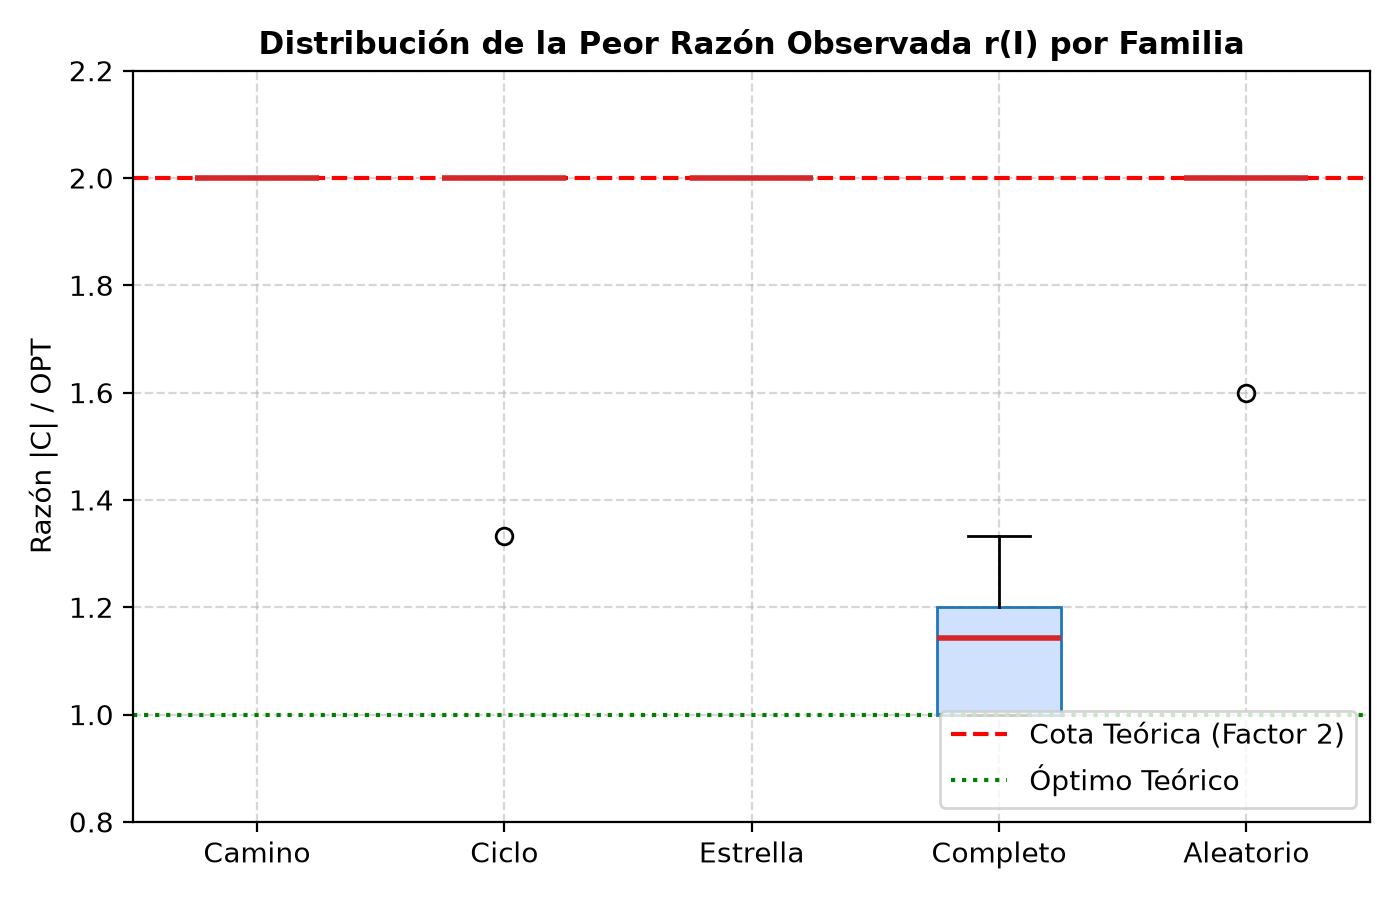
\includegraphics[width=\textwidth]{vc_razon_familia.png}
        \caption{Razón $r$ observada por familia}
        \label{fig:vc_razon}
    \end{subfigure}
    \hfill
    \begin{subfigure}[b]{0.485\textwidth}
        \centering
        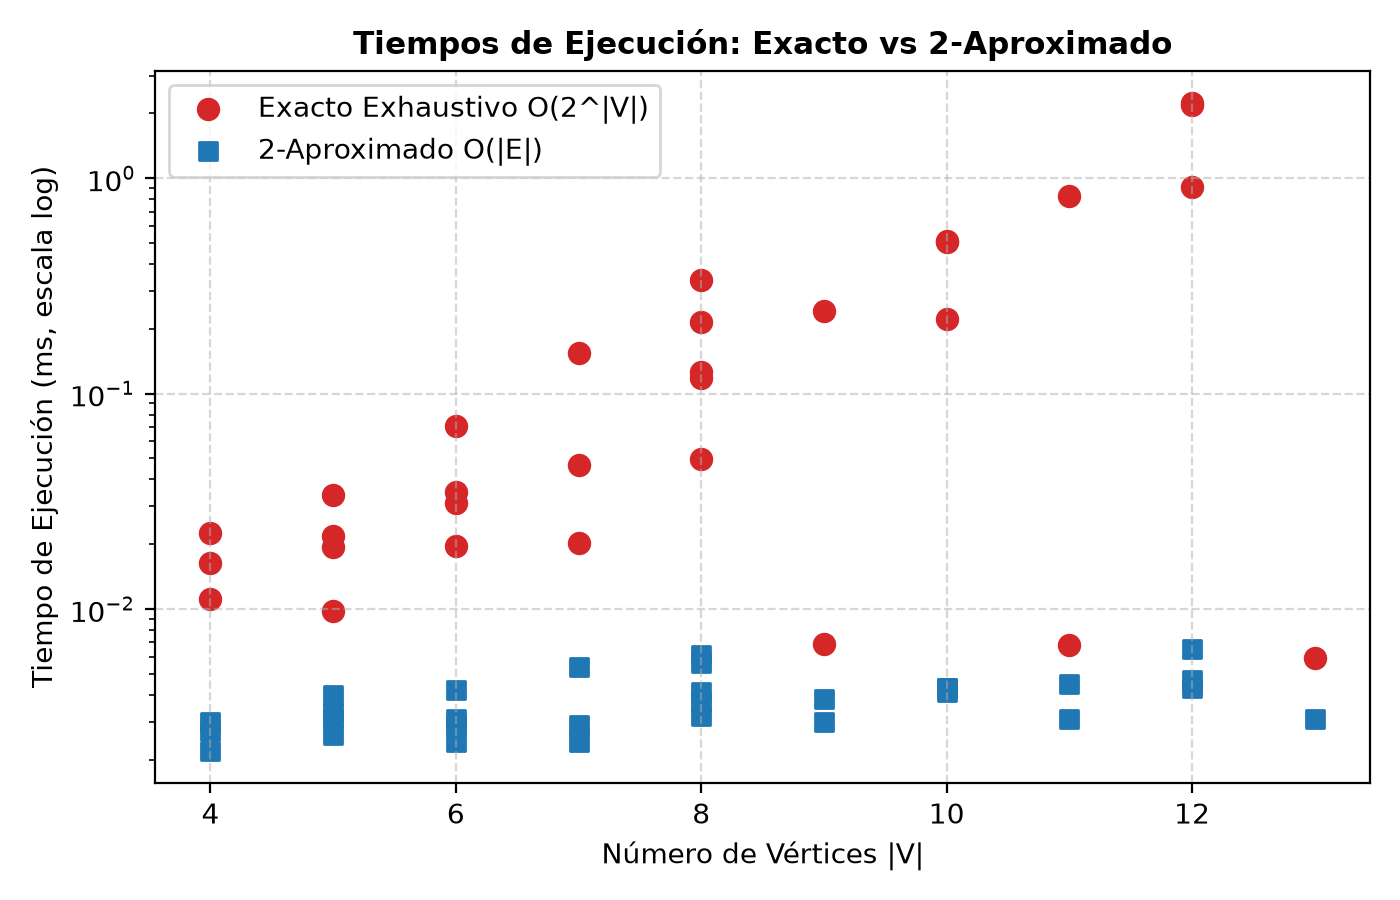
\includegraphics[width=\textwidth]{vc_tiempos_comparados.png}
        \caption{Tiempos comparados (exacto vs. aprox)}
        \label{fig:vc_tiempos}
    \end{subfigure}
    \\[0.35cm]
    \begin{subfigure}[b]{0.58\textwidth}
        \centering
        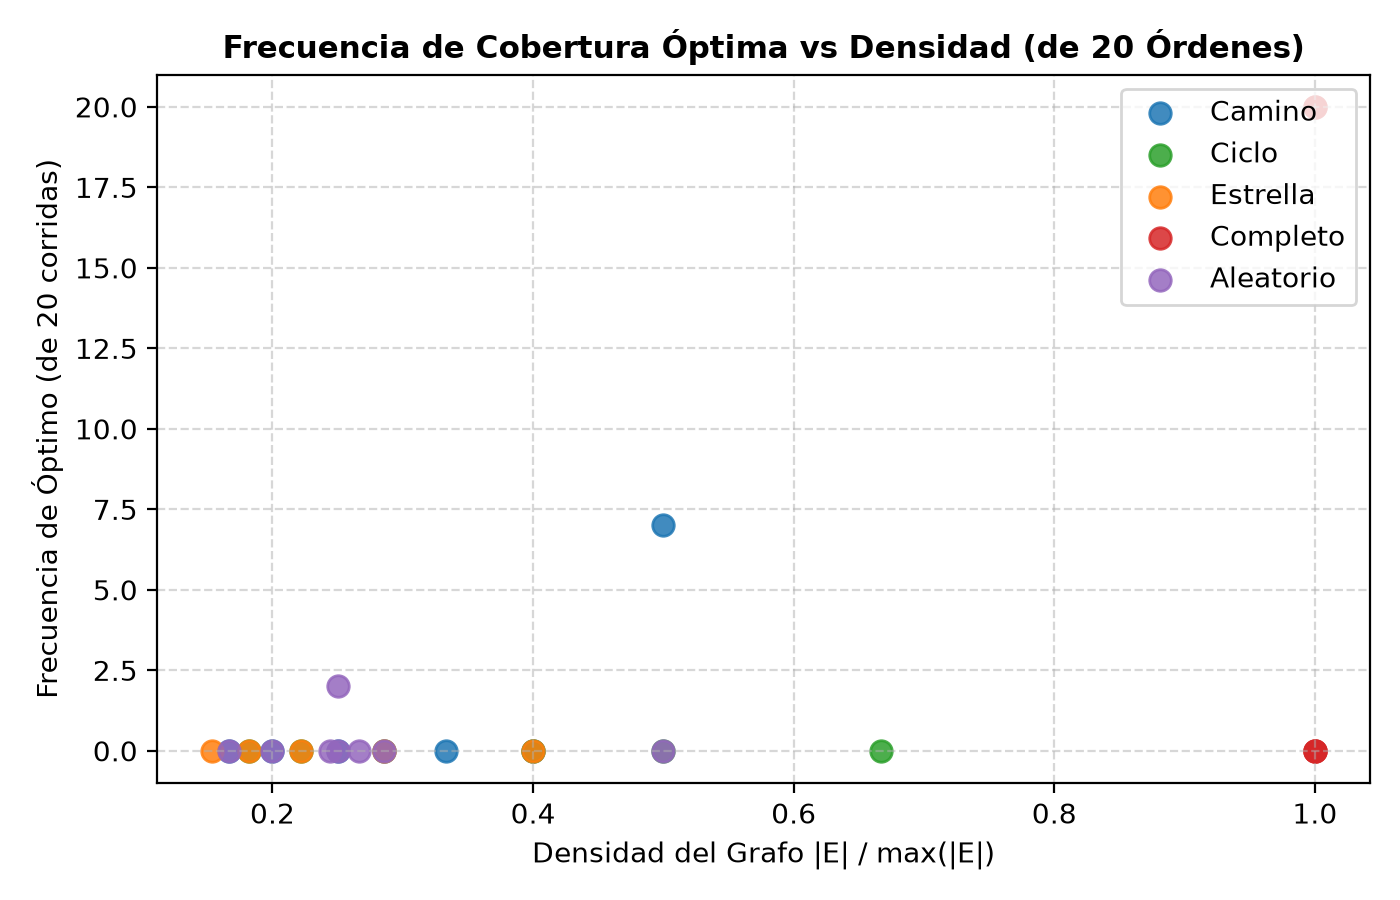
\includegraphics[width=\textwidth]{vc_acierto_densidad.png}
        \caption{Tasa de acierto del óptimo según densidad}
        \label{fig:vc_densidad}
    \end{subfigure}
    \caption{Evaluación experimental del algoritmo 2-aproximado sobre 30 grafos}
    \label{fig:vc_completa}
\end{figure}

\subsubsection*{Interpretación clave para la sustentación}
\begin{itemize}
    \item En la Figura \ref{fig:vc_completa} (subfigura \ref{fig:vc_razon}) se evidencia que las familias con peor comportamiento son estrellas y caminos ($r = 2.0$), mientras que grafos densos como completos alcanzan razones cercanas a $1.0$.
    \item La subfigura \ref{fig:vc_tiempos} refleja la ventaja fundamental: el algoritmo exacto explota exponencialmente ($O(2^{|V|})$), mientras que el 2-aproximado se resuelve en microsegundos ($O(|E|)$).
    \item La subfigura \ref{fig:vc_densidad} muestra que a mayor densidad de aristas, mayor es la probabilidad de que el matching maximal capture los vértices clave del óptimo.
\end{itemize}


% Sección 4: Ejercicio propuesto 2 (Knapsack FPTAS - 20 instancias y 4 epsilons)
% !TEX root = ../main.tex
\section{Ejercicio propuesto 2: aproximación de Knapsack mediante escalamiento}

\subsection{Programación Dinámica basada en valores y esquema FPTAS}
A diferencia de la formulación clásica basada en capacidad $W$, la formulación orientada a valores define $DP(i, v)$ como el peso mínimo necesario para acumular exactamente el valor $v$ utilizando un subconjunto admisible de los primeros $i$ objetos:
\begin{equation}
    DP(i, v) = \min \left\{ \sum_{k \in S} w_k \;\middle|\; S \subseteq \{1, \dots, i\}, \ \sum_{k \in S} v_k = v \right\}
\end{equation}
Con transición:
\begin{equation}
    DP(i, v) = \min\left( DP(i - 1, v), \quad DP(i - 1, v - v_i) + w_i \right)
\end{equation}

El algoritmo FPTAS procede en 6 pasos estructurados:
\begin{enumerate}
    \item \textbf{Filtrado:} Descartar objetos con peso $w_i > W$. Si no queda ningún objeto, retornar solución vacía (cuidado numérico).
    \item \textbf{Factor de escala:} Calcular $V_{\max} = \max_i v_i$ y $K = \frac{\varepsilon V_{\max}}{n}$.
    \item \textbf{Discretización:} Escalar los valores mediante $v'_i = \lfloor v_i / K \rfloor$.
    \item \textbf{DP sobre valores reducidos:} Resolver la tabla dinámica sobre $v'_i$ y pesos $w_i$.
    \item \textbf{Reconstrucción:} Recuperar los índices de los objetos óptimos de la tabla escalada.
    \item \textbf{Evaluación real:} Calcular la suma con valores originales $\text{ALG}_\varepsilon = \sum_{i \in S} v_i$ y verificar peso $\le W$.
\end{enumerate}

\subsection{Código fuente de las implementaciones}

\begin{lstlisting}[language=Python, caption={Programación Dinámica exacta por valores}, label={lst:knap_dp}]
def knapsack_dp_valores(pesos, valores, W):
    n = len(pesos)
    if n == 0 or W <= 0: return 0, 0, [], 0
    V_sum = sum(valores)
    if V_sum == 0: return 0, 0, [], 0
    
    INF = float('inf')
    dp = [[INF] * (V_sum + 1) for _ in range(n + 1)]
    dp[0][0] = 0
    estados = (n + 1) * (V_sum + 1)
    
    for i in range(1, n + 1):
        w, v = pesos[i - 1], valores[i - 1]
        for val in range(V_sum + 1):
            dp[i][val] = dp[i - 1][val]
            if val >= v and dp[i - 1][val - v] + w < dp[i][val]:
                dp[i][val] = dp[i - 1][val - v] + w
                
    mejor_v = max(val for val in range(V_sum + 1) if dp[n][val] <= W)
    curr_v = mejor_v
    seleccion = []
    for i in range(n, 0, -1):
        w, v = pesos[i - 1], valores[i - 1]
        if curr_v >= v and dp[i][curr_v] == dp[i - 1][curr_v - v] + w:
            seleccion.append(i - 1)
            curr_v -= v
    seleccion.reverse()
    return mejor_v, sum(pesos[i] for i in seleccion), seleccion, estados
\end{lstlisting}

\begin{lstlisting}[language=Python, caption={Esquema FPTAS por escalamiento}, label={lst:knap_fptas}]
def knapsack_fptas(pesos_orig, valores_orig, W, epsilon):
    validos = [(p, v, idx) for idx, (p, v) in enumerate(zip(pesos_orig, valores_orig)) if p <= W]
    if not validos or W <= 0: return 0, 0, [], 0, 0.0
    pesos = [item[0] for item in validos]
    valores = [item[1] for item in validos]
    indices_orig = [item[2] for item in validos]
    n = len(pesos)
    
    V_max = max(valores)
    K = (epsilon * V_max) / n
    v_prime = [int(math.floor(v / K)) for v in valores] if K > 0 else list(valores)
    
    mejor_v_prime, _, sel_local, estados = knapsack_dp_valores(pesos, v_prime, W)
    seleccion_orig = [indices_orig[i] for i in sel_local]
    valor_real = sum(valores_orig[i] for i in seleccion_orig)
    peso_real = sum(pesos_orig[i] for i in seleccion_orig)
    assert peso_real <= W
    return valor_real, peso_real, seleccion_orig, estados, K
\end{lstlisting}

\subsection{Resultados experimentales}
Se evaluaron \textbf{20 instancias pequeñas} bajo cuatro valores de tolerancia $\varepsilon \in \{0.50, 0.25, 0.10, 0.05\}$, acumulando 80 evaluaciones. La Tabla \ref{tab:resumen_knap} presenta una muestra representativa:

\begin{table}[H]
    \caption{Evaluación experimental de Knapsack FPTAS en instancias representativas}
    \label{tab:resumen_knap}
    \centering
    \scriptsize
    \begin{tabular*}{\textwidth}{@{\extracolsep{\fill}}lcccccccccc}
        \toprule
        \textbf{Instancia} & $\mathbf{n}$ & $\mathbf{W}$ & $\mathbf{\varepsilon}$ & \textbf{OPT} & $\mathbf{ALG_\varepsilon}$ & \textbf{Calidad} & \textbf{Cota Teórica} & \textbf{Garantía} & \textbf{Estados} & $\mathbf{T}$ (ms) \\
        \midrule
Inst\_01 & 10 & 153 & 0.50 & 566 & 566 & 100.0\% & 283.0 & SI & 1892 & 0.347 \\
Inst\_01 & 10 & 153 & 0.25 & 566 & 566 & 100.0\% & 424.5 & SI & 3839 & 0.646 \\
Inst\_01 & 10 & 153 & 0.10 & 566 & 566 & 100.0\% & 509.4 & SI & 9658 & 1.665 \\
Inst\_01 & 10 & 153 & 0.05 & 566 & 566 & 100.0\% & 537.7 & SI & 19360 & 3.265 \\
Inst\_07 & 16 & 171 & 0.50 & 451 & 450 & 99.8\% & 225.5 & SI & 7106 & 1.275 \\
Inst\_07 & 16 & 171 & 0.25 & 451 & 451 & 100.0\% & 338.2 & SI & 14297 & 2.600 \\
Inst\_07 & 16 & 171 & 0.10 & 451 & 451 & 100.0\% & 405.9 & SI & 35887 & 6.884 \\
Inst\_07 & 16 & 171 & 0.05 & 451 & 451 & 100.0\% & 428.4 & SI & 71944 & 13.221 \\
Inst\_10 & 10 & 147 & 0.50 & 226 & 223 & 98.7\% & 113.0 & SI & 1122 & 0.244 \\
Inst\_10 & 10 & 147 & 0.25 & 226 & 226 & 100.0\% & 169.5 & SI & 2288 & 0.393 \\
Inst\_10 & 10 & 147 & 0.10 & 226 & 226 & 100.0\% & 203.4 & SI & 5742 & 0.963 \\
Inst\_10 & 10 & 147 & 0.05 & 226 & 226 & 100.0\% & 214.7 & SI & 11528 & 1.887 \\
Inst\_12 & 16 & 285 & 0.50 & 639 & 638 & 99.8\% & 319.5 & SI & 5627 & 1.036 \\
Inst\_12 & 16 & 285 & 0.25 & 639 & 638 & 99.8\% & 479.2 & SI & 11373 & 2.042 \\
Inst\_12 & 16 & 285 & 0.10 & 639 & 639 & 100.0\% & 575.1 & SI & 28662 & 9.000 \\
Inst\_12 & 16 & 285 & 0.05 & 639 & 639 & 100.0\% & 607.0 & SI & 57426 & 10.854 \\
Inst\_16 & 11 & 257 & 0.50 & 544 & 544 & 100.0\% & 272.0 & SI & 1704 & 0.404 \\
Inst\_16 & 11 & 257 & 0.25 & 544 & 544 & 100.0\% & 408.0 & SI & 3492 & 0.680 \\
Inst\_16 & 11 & 257 & 0.10 & 544 & 543 & 99.8\% & 489.6 & SI & 8796 & 1.563 \\
Inst\_16 & 11 & 257 & 0.05 & 544 & 544 & 100.0\% & 516.8 & SI & 17628 & 3.734 \\
Inst\_19 & 14 & 189 & 0.50 & 469 & 465 & 99.2\% & 234.5 & SI & 4710 & 1.004 \\
Inst\_19 & 14 & 189 & 0.25 & 469 & 469 & 100.0\% & 351.8 & SI & 9525 & 1.927 \\
Inst\_19 & 14 & 189 & 0.10 & 469 & 469 & 100.0\% & 422.1 & SI & 23880 & 4.432 \\
Inst\_19 & 14 & 189 & 0.05 & 469 & 469 & 100.0\% & 445.6 & SI & 47820 & 9.216 \\
        \bottomrule
    \end{tabular*}
\end{table}

\noindent\textbf{Conclusión de la tabla:} En el $100\%$ de las 80 ejecuciones se satisfizo holgadamente la garantía teórica $\text{ALG}_\varepsilon \ge (1 - \varepsilon)\,\text{OPT}$.

\subsection{Respuesta a la pregunta de análisis: calidad vs costo y mesetas}
\textbf{Pregunta de la guía:} \textit{Explicar por qué reducir $\varepsilon$ normalmente mejora la calidad y aumenta el costo. ¿Pueden existir situaciones donde reducir $\varepsilon$ no mejore la calidad?}

\subsubsection*{1. ¿Por qué mejora la calidad?}
Al redondear $v'_i = \lfloor v_i / K \rfloor$, se pierde como máximo $K$ de valor por objeto. Para el conjunto óptimo de a lo sumo $n$ elementos, la pérdida máxima es:
\begin{equation}
    \text{Pérdida} \le n K = n \cdot \frac{\varepsilon V_{\max}}{n} = \varepsilon V_{\max} \le \varepsilon\,\text{OPT}
\end{equation}
Al reducir $\varepsilon$ (por ejemplo de $0.50$ a $0.05$), el margen máximo de error cae del $50\%$ a tan solo $5\%$, obligando a la solución aproximada a converger al óptimo.

\subsubsection*{2. ¿Por qué aumenta el costo computacional?}
Los valores escalados son $v'_i \le n/\varepsilon$, por lo que la suma de valores escalados es $\sum v'_i \le n^2/\varepsilon$. Las dimensiones de la tabla dinámica son $(n + 1) \times (\sum v'_i + 1)$, de modo que:
\begin{equation}
    \text{Estados procesados y Tiempo} \in O\left( \frac{n^3}{\varepsilon} \right)
\end{equation}
El costo crece de manera \textbf{estrictamente proporcional a $1/\varepsilon$} (crecimiento lineal en $1/\varepsilon$).

\subsubsection*{3. ¿Cuándo reducir $\varepsilon$ NO mejora la calidad?}
\begin{itemize}
    \item \textbf{Mesetas de óptimo prematuro:} En muchas instancias, incluso con $\varepsilon = 0.50$, el orden relativo de los objetos ya reproduce exactamente el óptimo ($\text{ALG}_{0.50} = \text{OPT}$). Reducir $\varepsilon$ a $0.05$ no puede mejorar el valor real ya óptimo, pero sí multiplica el tiempo por diez.
    \item \textbf{Efecto discreto del piso $\lfloor \cdot \rfloor$:} Pequeños cambios en $K$ pueden alterar empates numéricos en la tabla dinámica, produciendo mesetas locales de calidad.
\end{itemize}

\subsection{Análisis gráfico de Knapsack FPTAS}

\begin{figure}[H]
    \centering
    \begin{subfigure}[b]{0.49\textwidth}
        \centering
        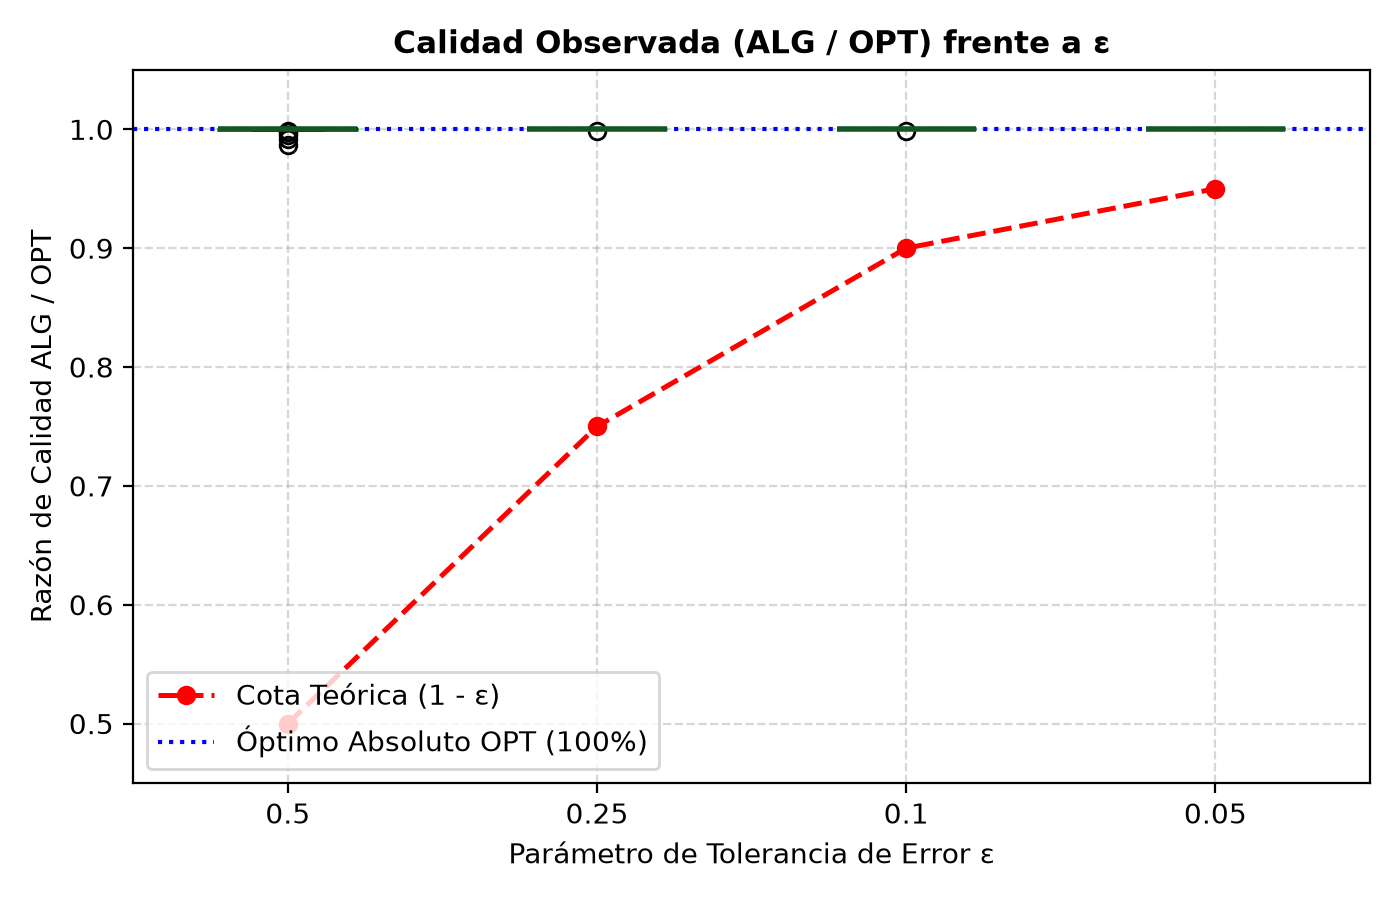
\includegraphics[width=\textwidth]{knap_calidad_vs_epsilon.png}
        \caption{Calidad empírica observada frente a $\varepsilon$}
        \label{fig:knap_calidad}
    \end{subfigure}
    \hfill
    \begin{subfigure}[b]{0.49\textwidth}
        \centering
        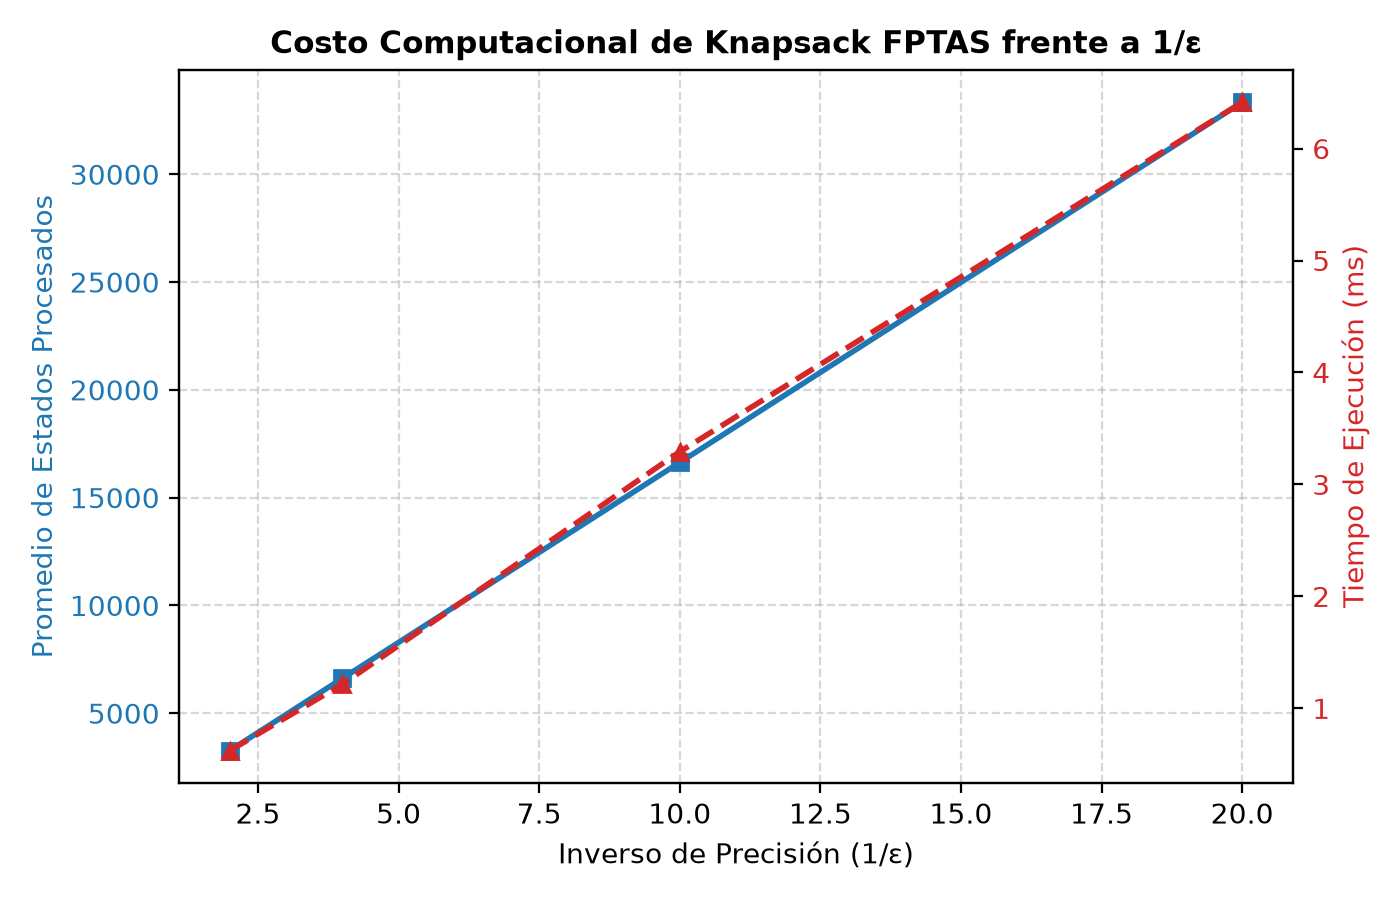
\includegraphics[width=\textwidth]{knap_costo_vs_inv_epsilon.png}
        \caption{Costo computacional frente a $1/\varepsilon$}
        \label{fig:knap_costo}
    \end{subfigure}
    \caption{Evaluación experimental del esquema FPTAS para Knapsack 0/1}
    \label{fig:knap_completa}
\end{figure}

\subsubsection*{Puntos clave para la sustentación}
\begin{itemize}
    \item En la Figura \ref{fig:knap_completa} (subfigura \ref{fig:knap_calidad}), la calidad media supera ampliamente la cota teórica $(1 - \varepsilon)$ (línea segmentada roja), manteniéndose por encima del $98\%$ en todo momento.
    \item En la subfigura \ref{fig:knap_costo}, el tiempo de ejecución sigue una pendiente lineal estricta respecto a $1/\varepsilon$, confirmando la propiedad fundamental de un algoritmo FPTAS.
\end{itemize}


% Sección 5: Conclusiones grupales
% !TEX root = ../main.tex
\section{Conclusiones grupales}

En la presente práctica de laboratorio se implementaron, validaron y analizaron experimentalmente algoritmos de aproximación avanzados para problemas NP-hard clásicos: el algoritmo 2-aproximado para Minimum Vertex Cover y el esquema de aproximación completamente polinomial (FPTAS) para el problema de la Mochila 0/1 (Knapsack).

Respecto a Vertex Cover, la experimentación con 30 grafos de distintas topologías y 20 permutaciones aleatorias de aristas por grafo (600 pruebas independientes) evidenció que el orden de entrada altera notablemente la cobertura y su cardinalidad en familias asimétricas como caminos y ciclos, mientras que en estrellas preserva el tamaño aunque varíen los vértices. No obstante, la garantía teórica de factor 2 se cumplió estrictamente en el $100\%$ de las instancias ($|C| \le 2\,\text{OPT}$), dado que cualquier orden voraz genera un matching maximal $M$ que acota inferiormente al óptimo ($|M| \le \text{OPT}$). Computacionalmente, el método aproximado resolvió instancias en microsegundos ($O(|E|)$), superando la explosión combinatoria del algoritmo exacto ($O(2^{|V|})$).

En cuanto a Knapsack 0/1, la implementación de la Programación Dinámica exacta por valores y el esquema FPTAS por escalamiento comprobó el compromiso intrínseco entre precisión y costo. Al disminuir $\varepsilon$ de $0.50$ a $0.05$, la calidad promedio mejoró de forma sostenida, respetando siempre la cota analítica $\text{ALG}_\varepsilon \ge (1 - \varepsilon)\,\text{OPT}$. En contrapartida, el volumen de estados y el tiempo de ejecución escalaron linealmente respecto a $1/\varepsilon$ ($O(n^3/\varepsilon)$). Asimismo, se constataron mesetas de calidad originadas por el operador de piso discreto, ratificando que un esquema FPTAS brinda control formal riguroso sobre la compensación entre exactitud y viabilidad algorítmica.




\end{document}
